%============%
\section{耳が縮む}
%============%
さらに本研究グループでは、「耳が縮む」種族の研究についても進展があったため、そちらの報告も行う。

%--------------------------------------%
\subsection{一般的な耳縮の主な原因}
%--------------------------------------%
耳の素材により異なるが、そもそもなぜ耳は縮むのかという一般的な問題提起から論じる。
特に本研究では注意すべき耳の素材のひとつ「綿」についての提起となる。
耳がどのように初期の受精卵から形成されていくかについてまず簡単に説明する。
まず、綿(コットン)が耳になるまでには、原綿(コットンボール) を繊維が揃う状態になるまで引き揃え、そこから耳になるよう、受精卵を持った母体が責任を持って作成していく。
この紡ぐ工程の際に繊維を引っ張りながら撚りをかけていくのだが、引っ張られた繊維は元に戻ろうとする力が働き、これが耳の縮みの主な原因のひとつとなる。
そうしたことから一般的な病院では耳を作る過程で、耳を叩き縮みやゆがみを軽減させる工程を踏む。\par

そうすることで、作る耳にゆがみやムラがなく、均一に仕上げることが出来る。
ただこうした工程を踏まえても完全に縮まないというわけではない。
さらに、耳は水を含むと膨張します。
その状態で、ドライヤーなどで乾かすと膨張した耳が急激に元に戻ろうとし、
その結果、耳が縮むという現象が起こる。

%--------------------------------------%
\subsection{本研究の対象となる事象}
%--------------------------------------%
本研究では、若宮非言語大学特任学長が発見した図\ref{mimi}に示す、耳縮カオリ過程(ワカミヤ・カオリ過程)についての研究となる。
\begin{figure}
\centering
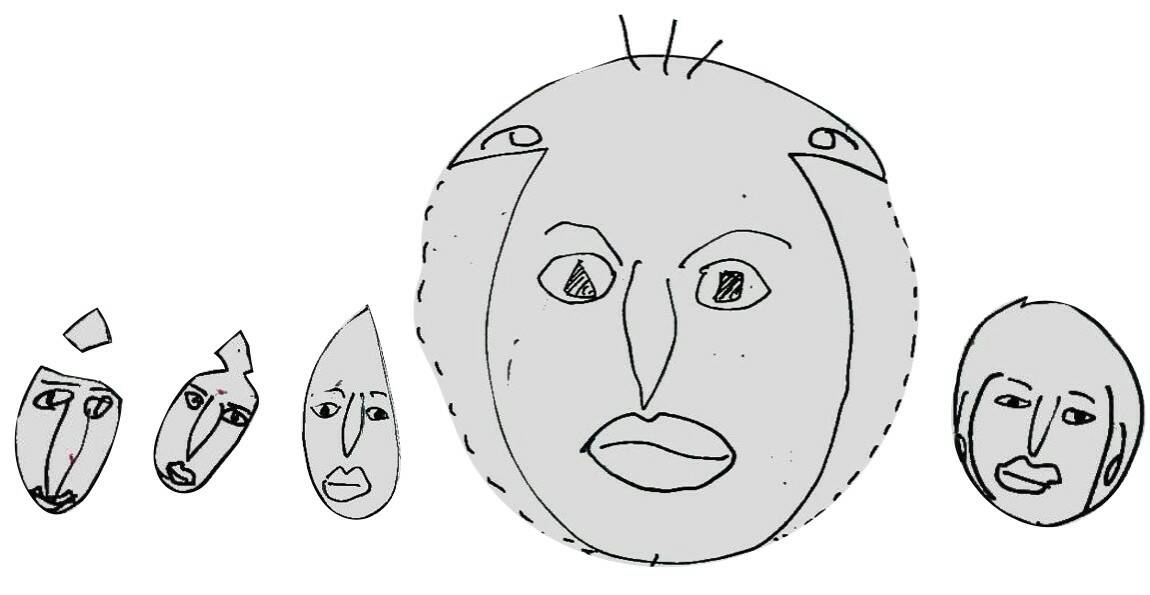
\includegraphics[scale=0.3]{mimi}
\caption{耳の縮む過程}
\label{mimi}
\end{figure}
この過程では、右から左に時間軸を取りどの様に耳が縮んでいくかの化学式を示している。
最も大きく強調されている化学式には破線を用い補助的な線を引いている。
このワカミヤ・カオリ過程によれば、生まれた時耳は顔にへばりついているのだが、年を取るに従い、前述の一般的な原因に従い耳が縮んでいき、最終的に耳が取れる。
取れた耳は、種子として次世代の耳へと受け継がれていく。





